\documentclass[12pt,oneside,a4paper]{article}

\usepackage[backend=biber,style=numeric]{biblatex}
\usepackage{float}
\usepackage{xcolor}
\usepackage{todonotes}
\usepackage{amsmath}
\usepackage{multicol}
\usepackage{caption}
\usepackage{pgfplots}
\usepackage{hyperref}
\usepackage{graphicx}
\usepackage{xcolor}
\graphicspath{{./imgs/}}
\usepackage{listings}
\DeclareCaptionFormat{listing}{\rule{\dimexpr\textwidth\relax}{0.4pt}\par\vskip1pt#1#2#3}
\captionsetup[lstlisting]{format=listing,singlelinecheck=false, margin=0pt,labelsep=space,labelfont=bf}

\usepackage{booktabs}
\usepackage[noabbrev,capitalise]{cleveref}
\crefname{listing}{algorithm}{algorithms}
\Crefname{listing}{Algorithm}{Algorithms}
\renewcommand\lstlistingname{Algorithm}
\def\lstlistingcrefname{Algorithm}
\usepackage{url}

\def\CC{{C\nolinebreak[4]\hspace{-.05em}\raisebox{.4ex}{\tiny\bf ++}}}

\addbibresource{biblio.bib}

\title{\textbf{Pynqrypt: a FPGA-accelerated encryption library for PYNQ}}

\author{FPGA101\\Roberto Alessandro Bertolini}

\date{\today}

\begin{document}

\begin{titlepage}
	\centering
	\clearpage
	\maketitle
	\thispagestyle{empty}
	\vspace*{1cm}
	\vfill
	\centering
	
\includegraphics{footer.png}
\end{titlepage}


\begin{abstract}
Data encryption and decryption is a computationally expensive task to perform, as most encryption algorithms aren't specifically optimized for running on modern computer architectures.
In this report we will analyze how a very common algorithm, AES-CTR, can be reimplemented on an FPGA to provide a noticeable improvement in throughput on low-power or embedded devices, shifting most of the operations to the FPGA and thus freeing up the main processor.
We will also note the various design considerations and the optimizations applied and how much they contributed to the overall improvement in throughput.
\end{abstract}

\section{Introduction} \label{sec:intro}
Nowadays cryptography is a fundamental part of our daily life: it is used to protect and ensure the integrity of our data, to authenticate users and to provide secure communications.
However, secure encryption and decryption protocols come at a high cost in terms of computational power required, a requirement which might become a bottleneck in many use cases, especially in low-power and embedded devices where energy efficiency or thermal constraints severely hinder hardware performance.
\\There are two different categories of cryptographic algorithms: symmetric and asymmetric.
Symmetric algorithms use the same key for both encryption and decryption, while asymmetric algorithms use a pair of two different keys, one for encryption and one for decryption.
Asymmetric algorithms are generally used for authentication and key exchange, while symmetric algorithms are used for the actual encryption and decryption of data.
The most common symmetric algorithm is the Advanced Encryption Standard (AES), which supersed the Data Encryption Standard (DES) in 2001 and became the de facto standard for symmetric encryption \cite{aes:development}.

\subsection{AES} \label{subsec:aes}
AES \cite{aes:specification} is a symmetric block cipher, which means that it encrypts data in blocks of a fixed size, which is 16 bytes (128 bits), with a key of 16, 24 or 32 bytes (128, 192 or 256 bits).
It is based on a substitution-permutation network: during the encryption process, the block is XORed, shifted, substituted or mixed byte-by-byte multiple times, in a reversible process that is easy to compute but hard to bruteforce without knowledge of the key used.
Since all of this is done using simple bitwise or mathematical operations, it can be easily ported to an FPGA, making it a perfect target for hardware acceleration.
\\AES only defines the method for encrypting a single block, but it doesn't specify how to chain multiple blocks together, which is the reason why it is usually used in conjunction with a mode of operation, which defines how to encrypt a stream of data.

\subsection{AES-CTR} \label{subsec:aes-ctr}
AES-CTR \cite{aes:ctr} is a mode of operation based on the AES algorithm. It is a stream cipher, meaning that it can encrypt a stream of data of any length, not necessarily a multiple of the block size, and it is based on a counter, which gets incremented at each block encryption.
A very important property of AES-CTR is that it is higly parallelizable, because each block can be encrypted and decrypted indipendently from the others, just by knowing the counter value of that specific block.
Another interesting behavior of AES-CTR is that the encryption and decryption operations are exactly the same, so the same code can be shared between the two.
This makes AES-CTR the perfect candidate for hardware acceleration, because the same IP can be reused for both encryption and decryption, and because its parallelizability is easily exploited by the FPGA.
\begin{figure}[h!]
	\centering
	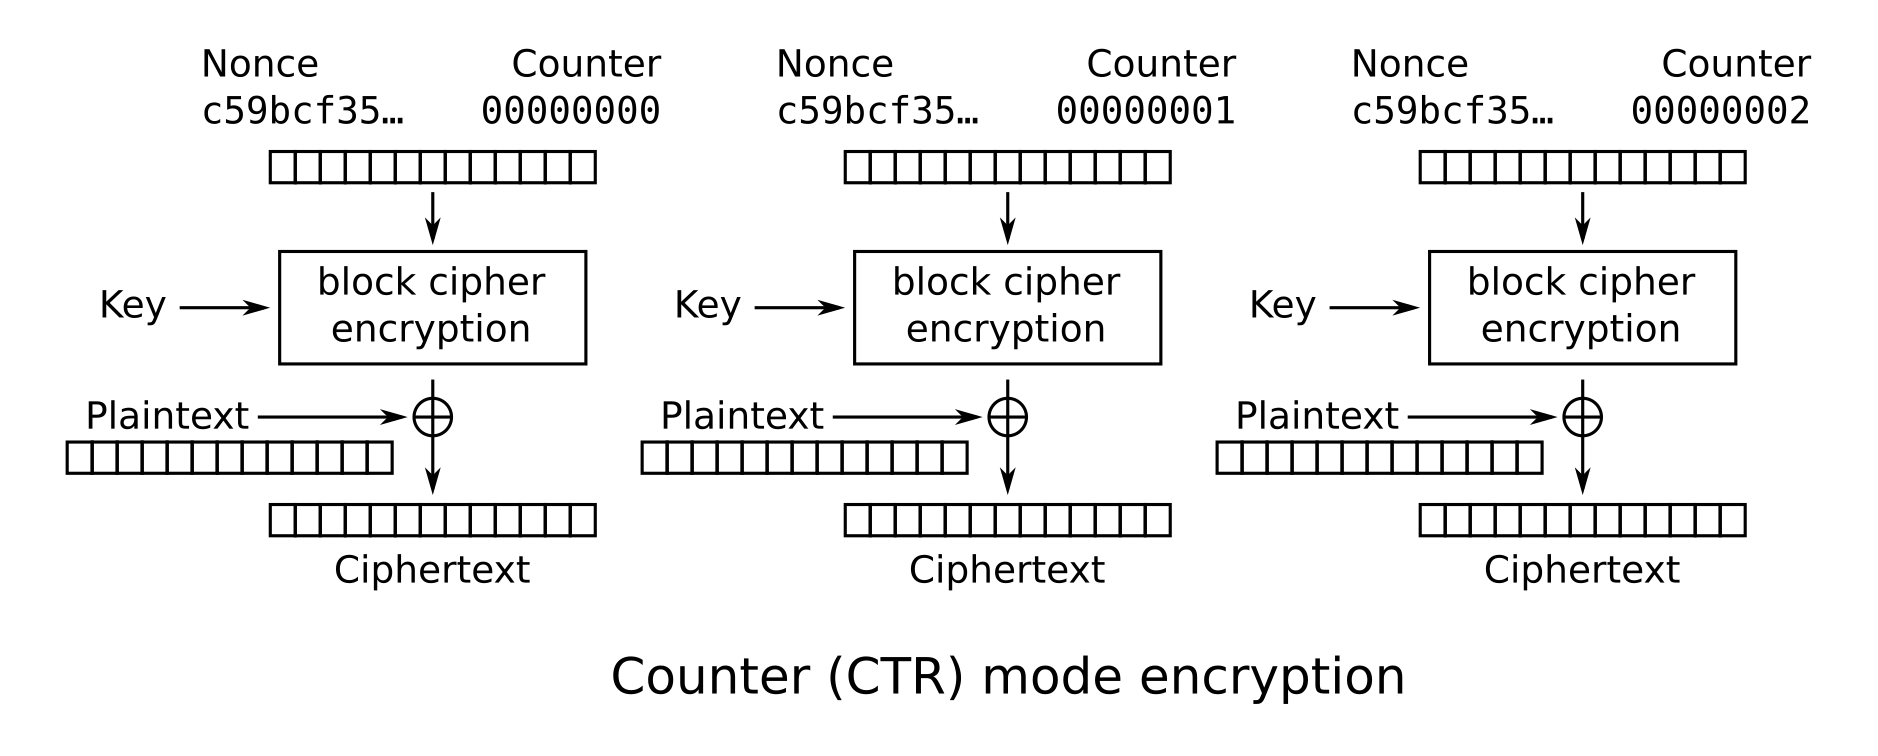
\includegraphics[width=\textwidth]{CTR_encryption_scheme.png}
	\caption{AES-CTR requires both a key and a nonce, which is a random value used to initialize the counter. For each block, the counter value is encrypted with the key, and the result is XORed with the plaintext to get the ciphertext. Then the counter is incremented by one. As XOR is its own inverse, the decryption flow is exactly the same, but Ciphertext and Plaintext switch places. \cite{pic:aes-ctr}}
\end{figure}

\subsection{The Hardware} \label{subsec:the-hardware}
The tests were conducted on a PYNQ Z2, an open-source development board for Xilinx Zynq SoCs, which features both a dual-core ARM CPU and a programmable FPGA fabric.
The CPU runs at 650 MHz and, unlike most modern designs, lacks the AES instruction set extensions \cite {aes:arm-extensions}, which makes it particularly slow at performing AES operations.
The FPGA runs at a variable frequency up to 250 MHz and is interconnected with the CPU via a high-speed AXI bus.
The board also features 512 Mbytes of DDR3 RAM, with a maximum bandwidth of 1050 Mbps, an Ethernet port, a microSD card slot, and other peripherals.

\section{Methodology} \label{sec:methodology}
Since the main goal of this project was to evaluate whether the FPGA is a viable alternative to the CPU when performing cryptographic operations with AES-CTR, the FPGA and the CPU were compared by measuring the time they took to perform the same operation on the same data with the same block key.
As in a real world scenario the data to be encrypted is usually of variable length, the tests were performed on a set of 4 different data sizes, which are:
\begin{enumerate}
	\item 16 bytes (1 block)
	\item 1024 bytes (64 blocks)
	\item 256 Kbytes (16 Kblocks)
	\item 16 Mbytes (1 Mblocks)
\end{enumerate}
The time measurements were repeated 10 times for each data size, and the average was then reported, excluding the highest and the lowest times.
\\As the FPGA IP would be used through the PYNQ Python API, we chose, for the sake of simplicity and consistency, to use a CPU implementation with Python bindings, which would enable us to run the benchmarks in the same environment, one after the other.
\\We chose the one provided by the PyCryptodome library, which, while exposing a Python API, implements the AES-CTR encryption flow in C and builds it from source code during the install process, so it should be able to leverage all the available architecture optimizations.
\\The FPGA implementation was written using Vitis HLS and the \CC language, and was then exported to Vivado as an IP, from which a bitstream was generated and downloaded to the FPGA.
Since a secondary goal of the project was to evaluate how easily a software implementation can be ported to hardware, we decided not to use any of the already existing AES-CTR libraries for the FPGA, but to write our own from scratch, starting from one that would work cross-platform.
With each iteration of our implementation, we tried to improve the hardware performance by optimizing the code, documenting which changes gave a positive or negative impact on the overall throughput.
To ensure the correctness of our code, at each iteration we validated the results against both the previously mentioned PyCryptodome library, and the OpenSSL library, which is widely trusted and used in many applications.
For brevity, we decided not to include iterations which didn't improve the performance significantly, nor to show code changes, but everything is available in the GitHub repository \footnote{\url{https://github.com/MrIndeciso/pynqrypt}} tagged by iteration version.
The benchmark results are available in the GitHub repository as well, in a single Jupyter notebook \footnote{\url{https://github.com/MrIndeciso/pynqrypt/blob/main/docs/results.ipynb}}, along with the source code for the Pynqrypt Python library and the \texttt{PynqryptTester} benchmark class.

\section{Design Iterations} \label{sec:iterations}

\subsection{Iteration 1} \label{subsec:iter1}
The first iteration of the design was very simple and intentionally generic. A few modifications had to be made to the original code, in order to make it compile in Vitis HLS:
\begin{enumerate}
	\item All the \CC standard library calls had to be replaced with C calls, as the HLS compiler does not support advanced \CC features like \texttt{std::copy}, which had to be replaced with \texttt{memcopy}.
	\item The original code defined a class, called \texttt{Pynqrypt}, which contained all the methods needed to perform the encryption and decryption operations. As Vitis HLS can expose only a single top-level function as a Vivado IP, we had to write a new function which just instantiates the \texttt{Pynqrypt} object and calls the appropriate methods on it before returning.
	\item A few interface pragmas had to be added to the previously mentioned function, so that the HLS compiler would know how to properly expose the function arguments in the generated IP. We opted for \texttt{m\_axi} ports for the input and output arrays, and \texttt{s\_axilite} ports for all the other arguments, as they don't need a high bandwidth interface.
\end{enumerate}

This first implementation achieved the following results:
\begin{table}[h!]
	\centering
	\begin{tabular}{ccc}
		\toprule
		 & CPU & Iteration 1 \\
		\midrule
		1 block & 0.11 ms & 0.16 ms \\
		64 blocks & 0.21 ms & 0.42 ms \\
		16 Kblocks & 24.52 ms & 67.86 ms \\
		1 Mblocks & 1641.08 ms & 4333.76 ms \\
		Max throughput & 78 Mbps & 29.54 Mbps \\
		\bottomrule
	\end{tabular}
\end{table}

As can be seen from the table, the FPGA is significantly slower than the CPU "out of the box", most likely due to the fact that the HLS compiler is not able to optimize the code much due to its intentionally generic nature.

\subsection{Iteration 4} \label{subsec:iter4}
This was the last fully cross-platform iteration.
In terms of optimization, we applied the following changes from Iteration 1:
\begin{enumerate}
	\item The functions {\tt Pynqrypt::ctr\_compute\_nonce}, {\tt Pynqrypt::ctr\_xor\_block}, {\tt Pynqrypt::aes\_mix\_columns}, {\tt Pynqrypt::aes\_shift\_rows}, \\ {\tt Pynqrypt::aes\_sub\_bytes} were inlined, to enable some pipeline optimizations.
	\item The loops in the {\tt Pynqrypt::aes\_mix\_columns} and {\tt Pynqrypt::aes\_sub\_bytes} functions were unrolled.
\end{enumerate}

These were all minor changes, so they didn't have a significant impact on the performance, but it is still worth mentioning them, as they are a good starting point for further optimizations and essentially cost-free.
The results of this iteration are the following:
\begin{table}[h!]
	\centering
	\begin{tabular}{cccc}
		\toprule
		 & CPU & Iteration 1 & Iteration 4 \\
		\midrule
		1 block & 0.11 ms & 0.16 ms & 0.16 ms \\
		64 blocks & 0.21 ms & 0.42 ms & 0.34 ms \\
		16 Kblocks & 24.52 ms & 67.86 ms & 45.91 ms \\
		1 Mblocks & 1641.08 ms & 4333.76 ms & 2928.72 ms \\
		Max throughput & 78 Mbps & 29.54 Mbps & 43.71 Mbps \\
		\bottomrule
	\end{tabular}
\end{table}

\subsection{Iteration 5} \label{subsec:iter5}
Iteration 5 saw a significant improvement in performance, mainly due to the switch from 16-element array of bytes to a 128 bit integer, implemented using the ap\_uint\textless128\textgreater type.
This change removed the need for a lot of loops in the code, which were previously used to perform bitwise operations on the array elements.
The downside of this change is that the code is now platform-dependent, as the ap\_uint type is specific to Xilinx FPGAs, and, as far as we know, closed source. Other than that, no further optimizations were made.

\begin{table}[H]
	\centering
	\begin{tabular}{cccc}
		\toprule
		 & CPU & Iteration 4 & Iteration 5 \\
		\midrule
		1 block & 0.11 ms & 0.16 ms & 0.17 ms \\
		64 blocks & 0.21 ms & 0.34 ms & 0.28 ms \\
		16 Kblocks & 24.52 ms & 45.91 ms & 33.08 ms \\
		1 Mblocks & 1641.08 ms & 2928.72 ms & 2107.78 ms \\
		Max throughput & 78 Mbps & 43.71 Mbps & 60.73 Mbps \\
		\bottomrule
	\end{tabular}
\end{table}

We expected to see a more significant improvement in performance in this iteration: either Vitis HLS was previously able to efficiently pipeline most of the loops, or something else is considerably slowing down our code.

\subsection{Iteration 6} \label{subsec:iter6}
Iteration 6 was the first to outperform the CPU implementation. The gains were achieved by optimizing the main loop function, removing a double copy of the data from the input buffer to the current block state.
This is due to the fact that ap\_uint internally stores the data in little endian format, but the AES algorithm expects the data to be big endian, so the block has to be reversed byte-by-byte before being encrypted, and then reversed again after the encryption.
This reversal was previously performed by copying the whole 16-byte block from the input buffer to the current block, then looping over it to reverse the endianness, keeping a temporary byte variable in order to perform the swap.
Now the reversal is performed by looping over the 16 bytes of the input array, and copying them to the current block in reverse order, thereby eliminating the need for the double copy. The same holds when copying the encrypted block back to the output buffer.

\begin{table}[H]
	\centering
	\begin{tabular}{cccc}
		\toprule
		 & CPU & Iteration 5 & Iteration 6 \\
		\midrule
		1 block & 0.11 ms & 0.17 ms & 0.15 ms \\
		64 blocks & 0.21 ms & 0.28 ms & 0.21 ms \\
		16 Kblocks & 24.52 ms & 33.08 ms & 24.72 ms \\
		1 Mblocks & 1641.08 ms & 2107.78 ms & 1573.01 ms \\
		Max throughput & 78 Mbps & 60.73 Mbps & 81.37 Mbps \\
		\bottomrule
	\end{tabular}
\end{table}

\subsection{Iteration 7} \label{subsec:iter7}
Iteration 7 saw a big jump in performance. 
During the AES encryption process, the 16 byte block has to be "substituted" multiple times by performing a byte-by-byte lookup in a 256-element constant array, which is called the S-box.
Previously Vitis HLS stored this array in a single BRAM, which meant that the lookup couldn't be performed in parallel, because the BRAM only has a single read port.
By applying the pragma "ARRAY\_RESHAPE" to the S-box array, we were able to split it into 256 single byte arrays, which occupy a BRAM each. With this change, the lookup can be performed in parallel, and the throughput increases significantly.
This change comes at no extra cost, because the Pynq board has 630K of fast BRAM available to be used, but in other devices, where no BRAM is available, it will have to be built using LUTs, increasing the footprint of the IP significantly.

\begin{table}[h!]
	\centering
	\begin{tabular}{cccc}
		\toprule
		 & CPU & Iteration 6 & Iteration 7 \\
		\midrule
		1 block & 0.11 ms & 0.15 ms & 0.16 ms \\
		64 blocks & 0.21 ms & 0.21 ms & 0.22 ms \\
		16 Kblocks & 24.52 ms & 24.72 ms & 19.16 ms \\
		1 Mblocks & 1641.08 ms & 1573.01 ms & 1216.49 ms \\
		Max throughput & 78 Mbps & 81.37 Mbps & 105.22 Mbps \\
		\bottomrule
	\end{tabular}
\end{table}

\subsection{Iteration 8} \label{subsec:iter8}
More lookup tables are used in the {\tt Pynqrypt::aes\_mix\_columns} function, which is used to perform the MixColumns step of the AES algorithm.
While lookup tables aren't strictly required in this step, they are there to avoid performing a lot of multiplications over Galois fields, which are computationally expensive.
The same limitations of the S-box apply here, so we applied the same pragma optimization.

\begin{table}[h!]
	\centering
	\begin{tabular}{cccc}
		\toprule
		 & CPU & Iteration 7 & Iteration 8 \\
		\midrule
		1 block & 0.11 ms & 0.16 ms & 0.16 ms \\
		64 blocks & 0.21 ms & 0.22 ms & 0.15 ms \\
		16 Kblocks & 24.52 ms & 19.16 ms & 7.60 ms \\
		1 Mblocks & 1641.08 ms & 1216.49 ms & 475.91 ms \\
		Max throughput & 78 Mbps & 105.22 Mbps & 268.96 Mbps \\
		\bottomrule
	\end{tabular}
\end{table}

The FPGA is now more than three times faster than the CPU on the largest data size, which is a huge improvement and would net a perceivable speedup in real-world applications.

\subsection{Iteration 9} \label{subsec:iter9}
For the last iteration we manually unrolled \texttt{Pynqrypt::aes\_sub\_bytes} just for the last encryption round, enabling some additional pipelining.
Having reached a result we were satisfied with, we decided to stop optimizing the code and we moved on to raising the clock frequency of the PL.
Even though Vitis HLS reported an estimated maximum design frequency of around 136 MHz, we found the IP to be stable up to 200 MHz, which is double the base frequency of the PL.
We decided not test the IP at the maximum supported frequency of 250 MHz because our aim was not to push the limits of the hardware, but to observe how the performance scaled with the clock frequency.
In a production environment we wouldn't recommend overriding the default clock frequency without adequate characterization of the IP, as it could lead to unexpected behavior.

\begin{table}[h!]
	\centering
	\begin{tabular}{cccc}
		\toprule
		 & CPU & Iteration 8 & Iteration 9 \\
		\midrule
		1 block & 0.11 ms & 0.16 ms & 0.15 ms \\
		64 blocks & 0.21 ms & 0.15 ms & 0.14 ms \\
		16 Kblocks & 24.52 ms & 7.60 ms & 6.80 ms \\
		1 Mblocks & 1641.08 ms & 475.91 ms & 427.36 ms \\
		Max throughput & 78 Mbps & 268.96 Mbps & 299.51 Mbps \\
		\bottomrule
	\end{tabular}
\end{table}

\begin{table}[h!]
	\centering
	\begin{tabular}{cccc}
		\toprule
		 & Iter. 9 (100 MHz) & Iter. 9 (143 MHz) & Iter. 9 (200 MHz) \\
		\midrule
		1 block & 0.15 ms & 0.16 ms & 0.15 ms \\
		64 blocks & 0.14 ms & 0.15 ms & 0.15 ms \\
		16 Kblocks & 6.80 ms & 5.44 ms & 4.66 ms \\
		1 Mblocks & 427.36 ms & 338.40 ms & 290.04 ms \\
		Max throughput & 299.51 Mbps & 378.25 Mbps & 441.31 Mbps \\
		\bottomrule
	\end{tabular}
\end{table}

We expected the throughput to scale linearly with the clock frequency, but the results show that the throughput actually increases at a slower rate.

\section{Results} \label{sec:results}
We can see from the previous table that the final iteration is able to vastly outperform the CPU implementation, especially for larger data sizes, with just a bit of tweaking and optimization, while causing only a small latency penalty for the smallest data size.
The results also show that the FPGA implementation is somehow bottlenecked by the system, as the throughput doesn't scale linearly with the increase in PL clock frequency.
We suspect that the culprit is the DDR3 memory, which, as we mentioned before, has a maximum bandwidth of 1050 Mbps. In order to achieve a throughput of 441 Mbps, we actually need to transfer data at a speed of 882 Mbps from and to the memory, which is close to that maximum bandwidth.

\section{Comparison with Other Hardware} \label{sec:conclusions}
We have successfully proven that the FPGA accelerator is a viable solution for accelerating AES-CTR encryption on the PYNQ Z2 board, but our hardware choice was particularly favourable to the aim of this report.
Modern x86\_64 and ARM CPUs have specific hardware instructions for performing AES encryption (\texttt{AES-NI} \cite{aes:aes-ni} o x86\_64 and \texttt{Cryptography Extensions} \cite{aes:arm-extensions} on ARM), which are orders of magnitude faster than the software implementation and much faster than our FPGA implementation.

\begin{table}[h!]
	\centering
	\begin{tabular}{cccc}
		\toprule
		 & Iter. 9 (200 MHz) & Ryzen 3 5300U \\
		\midrule
		1 block & 0.15 ms & 0.01 ms \\
		64 blocks & 0.15 ms & 0.01 ms \\
		16 Kblocks & 4.66 ms & 0.33 ms \\
		1 Mblocks & 290.04 ms & 22.45 ms \\
		Max throughput & 441.31 Mbps & 5.94 Gbps \\
		\bottomrule
	\end{tabular}
\end{table}

As we can see our FPGA is of no use in this scenario, but it is still a viable solution for other applications, such as embedded systems where the CPU is not powerful enough to perform the encryption in software, or where the CPU is already busy with other tasks.

\printbibliography

\end{document}


